\subsection{Notations}
For ease of presentation, we first define the following notation:
\begin{itemize}
\item $c_i$ denotes city $i$, or we sometimes
use $c$ to mean a generic city without specifying the subscript $i$. $\mathcal{T}$ denotes
a set of cities, which is expressed as $\mathcal{T}=\{c_i\}$. $N=|\mathcal{T}|$ denotes
the number of cities in $\mathcal{T}$. In this paper, without specification, $\mathcal{T}$ denotes
all the cities in South and Central America.
\item $P$ is a subset of $\mathcal{T}$, and can be denoted as $P\in 2^{\mathcal{T}}$.
\item $d(c_i,c_j)$ denotes the distance of node $c_i$ and $c_j$, and is normalized w.r.t. the maximal distance in $\mathcal{T}$.
\item $d(P)$ is the maximal distance in $P$, which is also the diameter of $P$.
\item $\alpha(c)$ denotes city $c$'s Twitter absenteeism score expressed in terms
of Z-scores.
Using a geocoded Twitter collection as a dataset, based on every day's Tweets volume,
we calculate each city's Z-score. A Z-score is defined as:
\begin{equation}
	\label{eq:zscore}
	\begin{array}{l}
		\alpha(c)=Zscore_t(n) =(X-\mu)/{\sigma}\,
	\end{array}
\end{equation}
where $X$ is the tweet volume at time interval $t$, $\mu$ is the trailing $n$-day moving average of the
tweet volume at time $t$, and $\sigma$ is the standard deviation of those trailing $n$-day moving Tweets volume at time $t$. We typically
use $Zscore(30)$ as a figure of merit.

\item $A$ is the area threshold, and is normalized by the whole area of South and Central America.
\item $d_{th}$ is the distance threshold.
\end{itemize}


\subsection{Miller cylindrical coordinate system.}
We converted the 3-dimensional spherical coordinate into a 2 dimensional
set of coordinates using the Miller cylindrical projection algorithms. %The conversion error is negligible because in most case the the size of $P_{min}$ is relatively small.
Since we are only interested in cities of Latin America, we set the center point of Latin
America as the original point in the Miller cylindrical coordinate system. Suppose that $c$'s latitude and longitude are $lat$ and $lon$; then $c$'s location in the Miller coordinate conversion can be written as:
\begin{equation}
x = lon - lon_0
\end{equation}
\vspace{-5mm}
\begin{equation}
y = 1.25*ln[tan(\frac{1}{4}\pi+\frac{2}{5}(lat-lat_0))],
\end{equation}
where $(lat_0,lon_0)$ is the center point of South American.
%Figure~\ref{fig:Brazil_regional_June20} plots the cities in the Miller cylindrical coordinate system.
In the rest of
this paper, all city locations refer to positions in the Miller cylindrical coordinate system.
\begin{figure}[t]
	\centering
	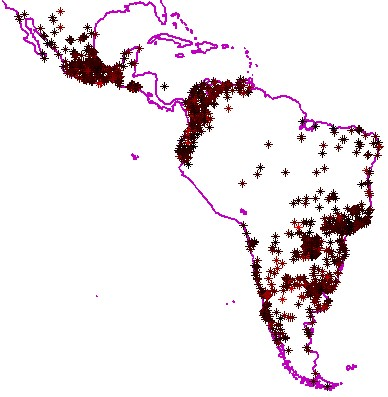
\includegraphics[width=1.5in]{figures/zscore.png}
	\caption{Absenteeism scores of 1290 cities in South American on May 16, 2014. One `*' point represents one city, and the darker the color is, the lower the its absenteeism score.}
	\label{fig:city_south_american}
\end{figure}


\subsection{Problem formulation}
 Figure~\ref{fig:city_south_american} plots the 1290 cities in Latin America
on May 16, 2014. Each city's absenteeism score is presented by its color. The darker the color is, the lower the city's absenteeism score is. We are interested with a city group, $P_{min}$ with the lowest absenteeism score. Usually, we require that all the cities in $P_{min}$ are close to each other. In this paper,  $P_{min}$ is required to meet one of the two constraints.

\paragraph{regional constraint} $P_{min}$ can be covered by
a convex polygon with areas less than $A$. With this constraint, we use $\Gamma_1(P)$ to denote $P$'s group absenteeism score, which can be expressed as:
 \begin{equation}
\Gamma_1(P)=\sum_{c_i\in H(P)} {\alpha(c_i)}
\end{equation}
The problem can be expressed as:

 \begin{equation}
 P_{min}=\argmin\limits_{P\in 2^\mathcal{T}, s(P)\leq A}\Gamma_1(P)
\end{equation}

 \paragraph{subgraph constraint}For any two cities in $P_{min}$, the distance between them is less than $d_{th}$. In this constraint, we use $\Gamma_2(P)$ to denote $P$'s group absenteeism score, which can be expressed as:
 \begin{equation}
\Gamma_2(P)=\sum_{c_i\in P} {\alpha(c_i)}
\end{equation}
The goal then is:
 \begin{equation}
 P_{min}=\argmin\limits_{P\in 2^\mathcal{T}, s(P)\leq A}\Gamma_2(P)
\end{equation}

